\documentclass[10pt,a4paper]{memoir}

\usepackage{a4wide}
\usepackage[utf8]{inputenc}
\usepackage{a4}
%\usepackage{geometry}
\usepackage[francais]{babel}
\usepackage{hyperref}
\usepackage{listings}
%\usepackage{latexsym}
%\usepackage{graphicx}
%\usepackage{appendix}
\usepackage{fancybox}
\usepackage{url}
\usepackage{graphics}
\usepackage{graphicx}
\usepackage{harvard}
\urlstyle{sf}
\makeatletter\def\input@path{{contenu/}{src/}{eps/}}\makeatother


\newcommand{\crypt}[2]{\begin{center}\texttt{#1}\ \ $\Longrightarrow$\ \ \texttt{#2}\end{center}}
\newenvironment{fminipage}%
  {\begin{center}\begin{Sbox}\begin{minipage}{1\textwidth}}%
  {\end{minipage}\end{Sbox}\fbox{\TheSbox}\end{center}}
\newcommand{\definition}[1]{\begin{center}#1\end{center}}
\renewcommand{\footref}[1]{\footnote{voir chapitre \ref{#1}, page
    \pageref{#1}}}
\newcommand{\note}[1]{\begin{center}\begin{minipage}{0.7\textwidth}\textsc{Note
          : }#1\end{minipage}\end{center}}
\newcommand{\bc}[1]{#1\ieme~ siècle avant J.-C.}


%\setlength{\voffset}{-0.9in}
%\setlength{\hoffset}{-0.5in}
%\setlength{\textwidth}{6.5in}
%\setlength{\textheight}{10.5in}

\title{Travail de fin d'études \\
  \textbf{La cryptographie} \\ 
  Peut on réellement cacher des informations ?}
\author{Quentin Stiévenart\\
Athéné Royal de Waterloo}
\date{Année scolaire 2008 - 2009}


%\pagestyle{headings}

\begin{document}
% Titre, table des matières
\frontmatter
\maketitle \clearpage
\tableofcontents \clearpage

% Introduction
\chapter{Introduction}
\thispagestyle{empty}

\section{Présentation du travail}
La cryptographie fait aujourd'hui partie de la vie de tous les jours,
on l'utilise sans le savoir, principalement en naviguant sur internet
(via les connexions sécurisées, les envois de mails chiffrés, \dots).

Mais qu'est-ce que la cryptographie ? Comment cela
fonctionne-t-il ? Son utilisation se limite-t-elle à l'informatique ?
Depuis quand existe la cryptographie ?

C'est à ces questions que nous allons essayer de répondre durant ce
travail, et plus principalement à celle-ci :

\begin{quote}
\emph{«~Peut-on réellement cacher des informations ?~»}
\end{quote}

Nous essayerons donc de savoir si l'on peut, et comment on peut 
envoyer sans risque une information, un message, des données, \dots à
quelqu'un, sans qu'une personne extérieure puisse le lire.

Pour répondre à ces questions, nous allons tout d'abord parler de
l'utilisation  de la cryptographie
à travers l'histoire, pour présenter ensuite les
différentes techniques existantes. Nous parlerons
aussi du moyen de « contrer » la cryptographie, avec la
cryptanalyse. Nous verrons enfin ce qu'il en est de la
cryptographie de nos jours. 

% La cryptographie est, comme le dit si bien Lacroix dans le titre de
% son livre ``La cryptographie, ou l'art d'écrire en chiffres''
% \cite{ArtDecrireEnChiffres},
% un ensemble de méthodes mathématiques ou autres, par lesquelles on va ``crypter'' un message, de façon à le rendre illisible si on n'a pas connaissance de la méthode utilisée, ou de l'éventuelle clée utilisée. \\
% Ce travail aura pour but de savoir si la cryptographie est un moyen fiable pour cacher des données, via l'analyse de certains algorithmes utilisés de nos jours ou dans le passé, et plus précisément leur cryptanalyse (ce terme sera définit à la prochaine section du document) \\
% Nous analyserons donc, d'abord les méthodes de cryptographie utilisée dans l'histoire, suivant un ordre chronologique, ensuite nous passerons aux méthodes actuelles, où nous expliquerons entre autres l'utilité de la cryptographie de nos jours. \\

%En annexe, on pourra voir quelques implémentations d'algorithmes de chiffrement dans certains langages de programmation (Haskell, C, Common Lisp, Python)\footnote{Pour plus d'infos sur ces langages, visitez respectivement \url{http://www.haskell.org}, \url{http://fr.wikipedia.org/wiki/Langage_C}, \url{http://cliki.net} et \url{http://www.python.org}.} \\

\section{Mes motivations pour ce travail}
J'ai choisi de faire un travail de fin d'études sur la cryptographie
car j'ai toujours été intéressé par les mathématiques et surtout par
l'informatique (plus le fonctionnement de l'ordinateur et sa
programmation, que l'aspect « jeux et divertissements » de
l'informatique, ainsi que la sécurité informatique)~;
la cryptographie fait partie intégrante des
systèmes informatiques d'aujourd'hui et est basée sur des principes
mathématiques. Je compte d'ailleurs faire des études polytechniques
l'année prochaine. \\ L'idée de ce travail m'est venue petit à
petit. Après la lecture d'un article sur la cryptographie sur
internet, j'ai commencé à m'y intéresser un peu, mais sans plus.
 Ce travail me permet donc d'approfondir le sujet.

\section{À propos de ce document}
Pour des raisons personnelles et dans un esprit de liberté de
l'information, ce document est placé sous licence Creative Commons
BY-SA\footnote{\url{http://creativecommons.org/licenses/by-sa/2.0/fr/}}, ce qui
signifie que vous pouvez le modifier et le redistribuer librement à
condition de préciser le nom de l'auteur, et de garder cette même
licence. Toujours pour les mêmes raisons, ce document a été préparé à
l'aide d'outils entièrement libres.
%de l'éditeur de texte \texttt{GNU
%  Emacs} et du logiciel de composition typographique \LaTeX, et des
%logiciels \texttt{xfig}, \texttt{dia} et \texttt{inkscape} pour les
%dessins, sur un système d'exploitation basé sur \texttt{Linux}. Tous
%ces logiciels sont entièrement libres. De plus, les langages utilisés
%en annexe possèdent aussi chacun au moins une implémentation
%libre.
Pour plus d'informations sur les logiciels libres et la culture
libre, référez-vous à \url{http://www.gnu.org/philosophy/philosophy.fr.html}. \\
Ce document, ses sources (les fichiers \TeX~, les graphiques, et les
codes sources des annexes), ainsi que des informations supplémentaires
sont disponibles sur internet via l'adresse
\url{http://www.acieroid.tuxfamily.org/crypto}. \\


\section{Présentation de la cryptologie}
Étymologiquement, la cryptologie est la «~science du secret~»~;
Elle consiste à cacher une
information, un message ou de quelconques données via la
\emph{cryptographie}. Nous étudierons son histoire
dans le chapitre \ref{chap:Histoire}.

La cryptographie comprend des méthodes très variées (des
\emph{systèmes de chiffrement} pour rendre les messages chiffrés)
avec certaines méthodes plus efficaces que les autres.
Nous examinerons ces méthodes dans le chapitre
\ref{chap:Techniques}.

La cryptologie comprend aussi la \emph{cryptanalyse}, qui consiste à
retrouver le message d'origine à partir d'un message chiffré sans en
connaître la clé ou le secret utilisé pour chiffrer le message.
Nous verrons cet aspect dans le chapitre \ref{chap:Cryptanalyse}.

Au cours de ce travail, nous utiliserons de nombreux termes se référant à
la cryptologie~; définissons-en quelques uns : 

%\newcommand{\glossaire}[2]{\nomenclature{\textbf{#1}}{#2}}
\begin{itemize}

\item {\sffamily\textbf{le chiffrement}} est la démarche effectuée afin de rendre
  le message clair illisible, chiffré. On utilise parfois le terme
  «~cryptage~», qui est un anglicisme~; nous éviterons donc de
  l'utiliser~;

\item {\sffamily\textbf{le déchiffrement}} est la démarche inverse du chiffrement, qui retrouve
  le message clair à partir du message chiffré en ayant connaissance
  de la clé, du secret ou de l'algorithme utilisé (contrairement à la
  cryptanalyse). Le mot {\sffamily\textbf{décryptage}} peut aussi
être utilisé~;
\item {\sffamily\textbf{la cryptanalyse}} vise à retrouver le
message clair à partir du message chiffré sans avoir connaissance
de la clé ou du secret~;

\item {\sffamily\textbf{la stéganographie}} est une discipline semblable à la
  cryptographie mais qui consiste à cacher un message (dans une
  image\dots) et non pas à la rendre inintelligible. Nous ne
développerons donc pas ce sujet ici~;

\item {\sffamily\textbf{la clé de chiffrement}} est une donnée (mot, suite d'opération,
  nombre\dots) utilisée pendant le chiffrement afin de rendre le
  déchiffrement plus difficile sans la connaissance de celle-ci. Il
  existe plusieurs types de clés : certaines qui doivent être gardées
  secrètes (clés privées) et d'autres qui peuvent être diffusées
  (clés publiques)~;

\item {\sffamily\textbf{les données claires}} sont les données dans leur forme initiale, non
  chiffrées. Ces données peuvent être du texte (un message) ou d'autres
  données informatiques (un fichier,\dots)~;

\item {\sffamily\textbf{les données chiffrées}} sont les données qui
sont chiffrées via un certain
  algorithme de chiffrement~;

\item {\sffamily\textbf{un cryptogramme}} est un message chiffré
dans le but d'être déchiffré par des amateurs de cryptographie (on
en retrouve par exemple dans les journaux). Ils sont la plupart du
temps assez simples.
\end{itemize}



% Partie principale
\mainmatter

\chapter{Présentation de la cryptologie}
\section{Qu'est ce que la cryptologie}
La cryptologie est la « science du secret », et consiste a cacher une
information, un message, ou de quelconques données via la
\emph{cryptographie}. 

Elle comprends aussi la \emph{cryptanalyse}, qui consiste à retrouver
le message d'origine à partir d'un message chiffré, sans en connaître
la clé ou le secret utilisé pour chiffrer le message.
\section{Vocabulaire\label{s:Definitions}}
Avant toute chose, il est nécéssaire de définir quelques termes pour
les clarifier dans l'esprit de chacun, et pour éviter de les confondre
:
\begin{itemize}
\renewcommand{\makelabel}[1]{\sffamily\textbf{#1}}
\item[Le chiffrement] se réfère à la démarche effectuée afin de rendre
  le message clair illisible, chiffré. On utilise parfois le terme
  « cryptage », qui est un anglicisme, nous éviterons donc de
  l'utiliser ;

\item[Le déchiffrement, ou décryptage] est le sens inverse du
  chiffrement, qui retrouve le message clair à partir du message
  chiffré, en ayant connaissance de la clé, du secret ou de
  l'algorithme utilisé (contrairement à la cryptanalyse). Le terme
  « décryptage » est un terme français correct, contrairement au
  « cryptage » ;

\item[La stéganographie] est une discipline semblable à la
  cryptographie, mais qui consiste à « cacher » un message (dans une
  image, ...) et non pas à le rendre inintelligible. Ce sujet étant
  tout aussi vaste que la cryptographie, nous ne l'étudierons pas dans
  ce travail ;

\item[La clé de chiffrement] est une donnée (mot, suite d'opération,
  nombre, ...) utilisée pendant le chiffrement afin de rendre le
  déchiffrement plus difficile sans la connaissance de celle ci.
  Nous verrons qu'il existe deux types de clés : \emph{symétrique}
  (\emph{privées}) et \emph{asymétrique} (\emph{publiques}), et que
  l'utilisation de clé est crucial dans la cryptographie actuelle.
\end{itemize}

\section{Règles typographiques}
Tout au long de ce travail, nous allons utiliser certaines notations : 
\begin{itemize}
\item Une \textbf{clé de chiffrement} sera notée $k$ (pour «  Key  »,
  «  Clé  » en anglais), indicé si nous utilisons plusieurs clés ;
  \item Un \textbf{message en clair} sera noté $M$ (pour «  Message  ») ;
  \item Un \textbf{message chiffré} sera noté $C$ (pour «  Chiffré  ») ;
  \item Une \textbf{fonction de chiffrement} $e$ (pour « Encryption
    », «  Chiffrage  » en anglais) ou $e_k$, selon qu'elle utilise
    une clé pour le chiffrement ;
  \item Une \textbf{fonction de déchiffrement} $d$ (pour
    « Decryption », « Déchiffrement  » en anglais) ou $d_k$,
    similairement à la fonction de chiffrement.
\end{itemize}
L'opération de chiffrement se notera alors comme suit pour un
algorithme de chiffrement avec une clé.
\begin{center}
  \begin{math}
    e_k(M) = C
  \end{math}
\end{center}
Et l'opération de déchiffrement se notera ainsi :
\begin{center}
  \begin{math}
    d_k(C) = M
  \end{math}
\end{center}
Nous utiliserons aussi la notation : 
\crypt{Cryptographie}{Pelcgbtencuvr}
pour indiquer que le mot « Cryptographie » sera chiffré en
 « Pelcgbtencuvr ». 
  

\chapter{La cryptographie à travers l'histoire\label{chap:Histoire}}
\thispagestyle{empty}
Avant de décrire la cryptographie en soi, passons en revue
son histoire, son apparition et son évolution au fil du temps ; les
aspects techniques brièvement présentés dans ce chapitre seront
expliqués au cours des chapitres suivants.

\section{L'apparition de la cryptographie}
La cryptographie serait apparue pour la première fois il y a 4000 ans,
au bord du Nil ~: un scribe aurait tracé d'une façon particulière des
hiéroglyphes sur la tombe de son maître. Le but n'était néanmoins
pas de rendre le texte illisible, mais de le rendre plus solennel.

La seconde trace de cryptographie date du \bc{XVI}. Il s'agit d'une tablette
d'argile sur laquelle un potier aurait écrit sa recette en enlevant
les consonnes et en changeant l'orthographe de certains mots. \\

À cette époque-là, les seuls moyens utilisés pour cacher les messages
ressemblaient plus à de la stéganographie qu'à de la cryptographie
~;
les messages ne sont pas rendus illisibles, mais sont cachés. Par
exemple, durant le \bc{VII}, Nabuchodonosor rasa le crâne d'un
esclave, écrivit un message dessus et une fois que les cheveux
eurent repoussé, envoya l'esclave chez le destinataire du message,
qui à son tour rasa les cheveux pour le lire. Un autre exemple est celui
d'Harpage, qui avait été chargé de tuer Cyrus, le petit-fils du roi de
Mèdes, mais qui ne le fit pas. Par la suite, quand Cyrus eut
grandi,
pour communiquer avec lui, Harpage cachait les lettres dans le ventre
de lièvres, qu'il recousait ensuite. De cette façon, les messages
passaient
inaperçus. \\

Les premières «~vraies~» techniques de cryptographie apparurent,
quant à elles, à partir du \bc{VI}, avec une méthode de substitution,
nommée \emph{atbash}. Celle-ci consiste à remplacer les lettres par la
lettre « opposée », c'est-à-dire que A sera remplacé par Z, B par Y,
et ainsi de suite.
\begin{figure}[h]
%\begin{wrapfigure}{l}{0.5\textwidth}
  \centering
%    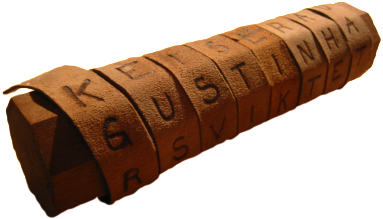
\includegraphics[scale=1]{images/Scytale.png}
%    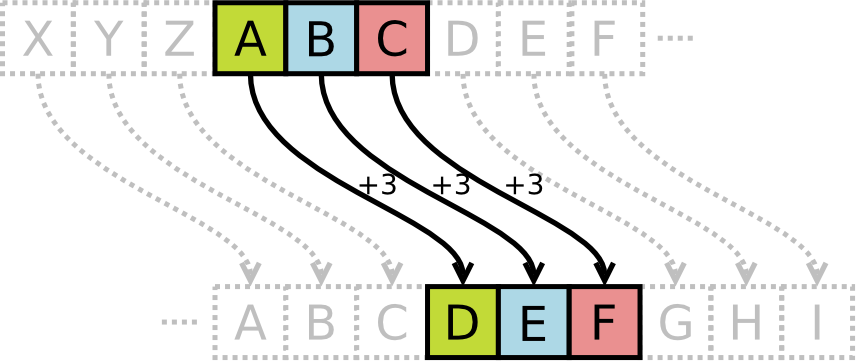
\includegraphics[scale=0.4]{images/ChiffreCesar.png}
    \subfloat[La scytale des Spartiates.]{
      \label{fig:Scytale}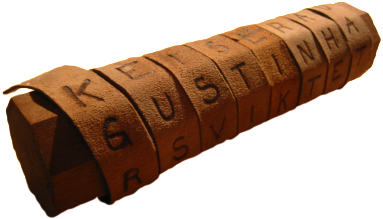
\includegraphics[width=0.4\textwidth]{images/Scytale.png}}
    \hspace{1.5cm}
    \subfloat[Le fonctionnement du chiffre de César.]{
      \label{fig:Cesar}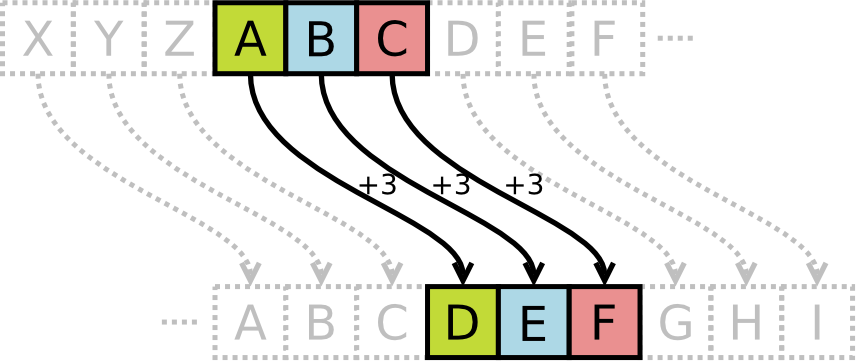
\includegraphics[width=0.4\textwidth]{images/ChiffreCesar.png}}
%    \vspace{-5pt}
    \caption{deux anciennes techniques de chiffrement.}
    \vspace{-15pt}
%  \label{fig:ScytaleChiffreCesar}
\end{figure}
%\end{wrapfigure}
% \begin{figure}[h]
%   \begin{center}
%     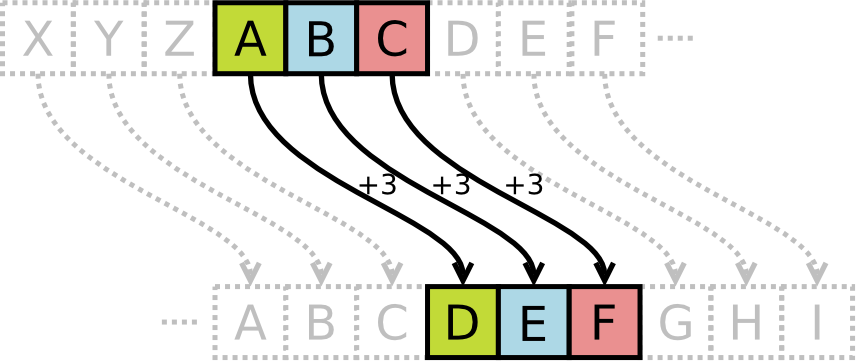
\includegraphics[scale=0.4]{images/ChiffreCesar.png}
%   \end{center}
%   \caption{Le chiffre de César}
%   \label{fig:ChiffreCesar}
% \end{figure}


  
Ensuite, au \bc{V}, les Spartiates utilisaient, pour communiquer, le
bâton de Plutarque, plus connu sous le nom de \emph{scytale}. Cette
technique consistait à enrouler un long et étroit morceau de parchemin
autour d'un bâton, on écrivait ensuite le message sur le parchemin et
on envoyait ce parchemin déroulé au destinataire, qui possédait un
bâton de même diamètre pour déchiffrer le message.

Le premier réel système cryptographique par substitution fut inventé
par un historien grec, Polybe aux alentours de 150 avant J.-C. (nous
verrons ce système en détail dans le chapitre \ref{syst:CarrePolybe} (page
\pageref{syst:CarrePolybe}). \\

\label{syst:ChiffreCesar}
Pendant le \bc{I}, les armées de César utilisaient une méthode de
chiffrement par substitution simple qui consistait à décaler les
lettres de l'alphabet d'un certain rang dans l'alphabet (de 3 rangs la
plupart du temps, ainsi A devient D, B devient E, \dots). Cette 
méthode simple est une des méthodes de chiffrement les plus
connues. Elle a été
utilisée de nombreuses fois par la suite dans des formes dérivées (chiffre de
Vigenère\footref{syst:ChiffreVigenere}, rot13\footref{syst:rot13}), ou même
de la façon identique (pendant la guerre de Sécession par exemple).

Au Moyen Âge, comme la plupart des sciences, la cryptologie n'évolua
presque pas (une personne pratiquant la cryptologie peut être
considérée comme faisant de la magie noire), à part quelques exceptions
au Moyen-Orient et en Asie (dans le \emph{Kama-sutra}, il est dit que les
femmes doivent apprendre le \emph{mlecchita-vikalpa} (l'art de
l'écriture secrète) pour cacher leurs liaisons.). Il faudra donc
attendre le XV\ieme~siècle pour que la cryptographie commence
réellement à évoluer. \\

\section{L'évolution de la cryptographie}
Au début du XV\ieme~siècle donc, un Égyptien écrit une encyclopédie
en 24 volumes comprenant une partie sur la cryptologie. Il y décrit des
chiffres de substitution et de transposition. Le premier chiffre de
substitution polyalphabétique\footref{SubstitutionPolyalphabetique}
est inventé par Leone Battista Alberti en 1467, un humaniste italien
de la Renaissance, aussi connu pour ses travaux en architecture et
surnommé \emph{Le père de la cryptographie occidentale} par
l'historien David Kahn \cite{Codebreakers}. Cette technique est appelée
le \emph{cadran chiffrant}\label{syst:CadranChiffrant}~; elle consiste
en deux disques attachés ensemble de façon à pouvoir coulisser,
chacun d'eux contenant les lettres de l'alphabet dans 24 cases (le premier
en contient 20, H, K et Y n'étant pas « indispensables », J, U et W
n'étant pas dans l'alphabet latin, les 4 autres cases sont occupées
par des chiffres. L'autre disque contient les 23 lettres latines dans
un ordre aléatoire et le signe \texttt{\&}). Le plus petit disque peut tourner,
les lettres claires et chiffrées se trouvent alors face à face, et il
suffit de recopier la lettre du petit disque pour chiffrer la lettre
du grand disque. Après avoir chiffré quelques lettres, on décale le
disque et on continue ainsi de suite, en indiquant sur le message
chiffré le changement. Dans son ouvrage, il parle aussi de
cryptanalyse, et il introduit le concept d'analyse des
fréquences. \\

\begin{figure}[h]
  \begin{center}
    \subfloat[Le cadran chiffrant d'Alberti dans sa forme
originelle.]{
      \label{fig:CadranChiffrant}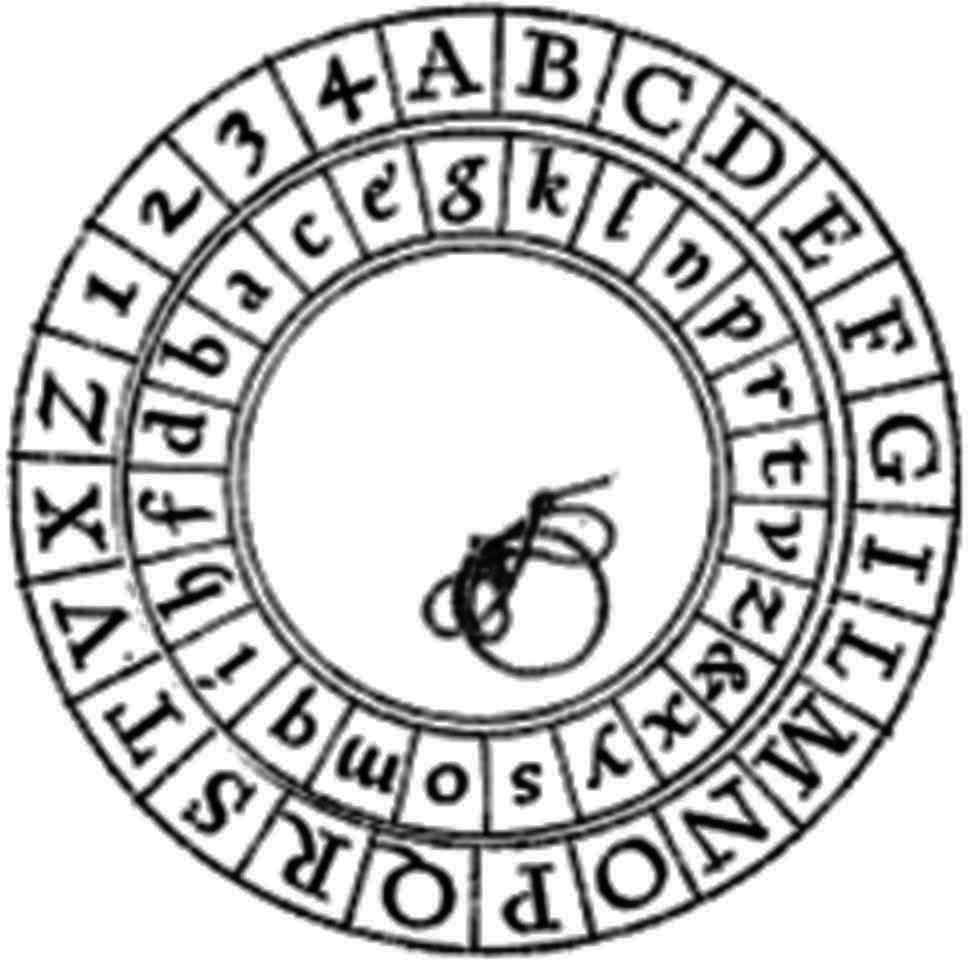
\includegraphics[width=0.4\textwidth]{images/AlbertiCipherDisk.jpg}}
    \hspace{1.5cm}
    \subfloat[Le cadran chiffrant réutilisé par les confédérés pendant
    la guerre de sécession.]{
      \label{fig:CadranConfederes}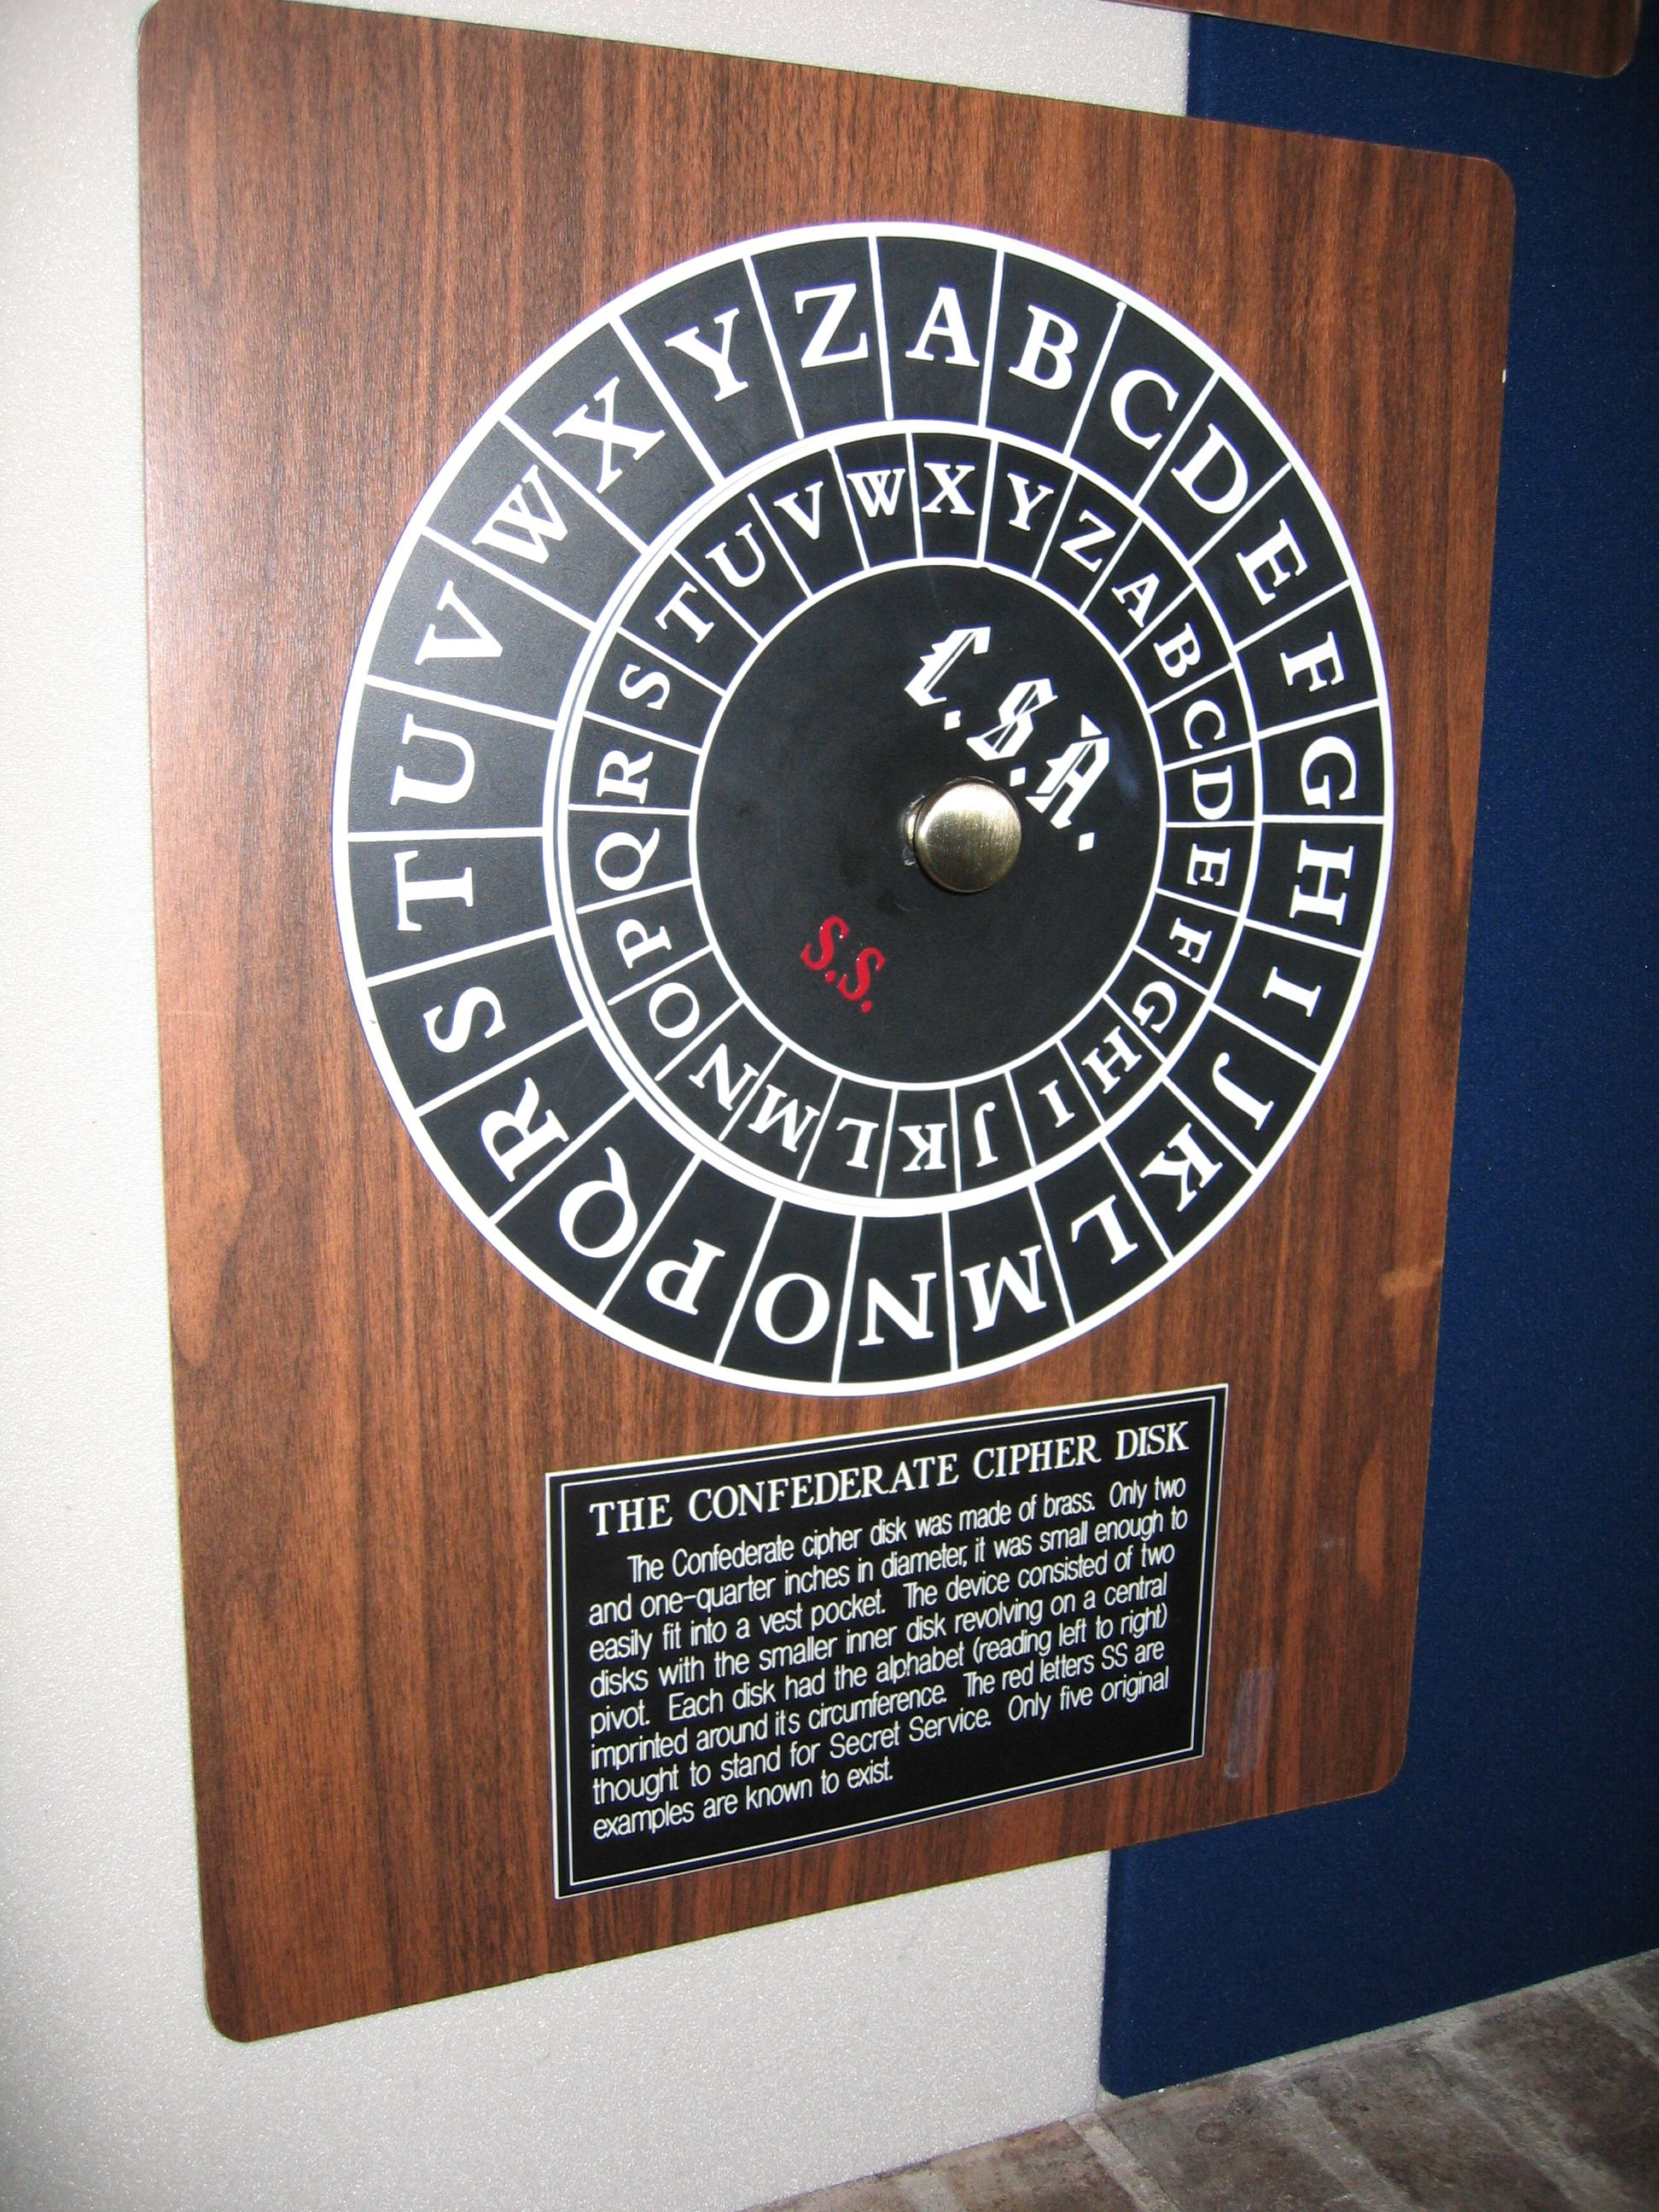
\includegraphics[width=0.4\textwidth]{images/ConfederateCipherDisk.jpg}}

  \end{center}
  \vspace{-10pt}
  \caption{cadrans chiffrants.}
  \vspace{-15pt}
\end{figure}

En 1518, Jean Trithème publie \emph{Polygraphi\ae} , le premier livre imprimé
sur la cryptologie, où il invente un chiffre stéganographique,
ainsi que ce
qui deviendra par la suite le chiffre de
Vigenère. \\

Au milieu du XVI\ieme~siècle, Jérôme Cardan invente le premier
\emph{procédé autoclave} (qui utilise le message clair comme clef),
mais ce système comporte des lacunes. Il invente aussi la \emph{grille
  de Cardan}, un système stéganographique qui cache un message dans
une grille de lettres. Pour lire le message, il faut utiliser un cache
troué d'une certaine façon, les lettres apparaissent alors dans les
trous, et on peut lire le message. \\

%\begin{figure}[h]
\begin{wrapfigure}{L}{0.5\textwidth}
  \begin{center}
    \includegraphics[scale=0.2]{images/GrilleCardan.png}
  \end{center}
  \caption{un exemple de grille de Cardan.}
  \label{fig:GrilleCardan}
  \vspace{-10pt}
%\end{figure}
\end{wrapfigure}

% Premières techniques de cryptographie
% Plus vieux document chiffré : un potier qui écrit sa recettes en
% enlevant des consonnes et en changeant l'orthographe des mots.
% En chine : stégano (papirus enroulé en boule recouvert de cire, avalé)
% première trace : vers 2000 av J.-C.
% Scytale -500 av J.-C. : == bâton de Plutarque.
% Spartiates, bâton rond, qu'on entoure d'un long et étroit morceau de
% parchemin. Une fois mis autour, on écrit le message dessus, puis on
% l'envoie au destinataire, qui possède une scytale de même diamètre,
% et qui déchiffre donc facilement le message. Fa
% Nabuchodonosor : -600 av J.-C. : 
% On rase le crâne d'un esclave, et une fois les cheveux repoussés, on
% l'envoie au destinataire, qui rase à nouveau les cheveux.
% Harpage qui envoie un message à Cyrus, il ouvre le ventre d'un
% lièvre pour y cacher une lettre, et l'envoya à Cyrus.
% Hebreux : Vieme av JC, atbash, chaque lettre est inversée A->Z,
% B->Y, ...

% ~-200 : premiers "vrais" systèmes cryptographiques : 
% caré de polybe, historiengrec : ~-150
% 1er siècle avant J.-C. : 
% code de césar utilisé dans l'armée romaine, réutilisé par la suite
% durant la guerre de sécession et l'armée russe en 1915 (rot13)

% Moyen age : quasi rien car sorcellerie, tout ça.

% Quasi rien jusqu'au XVieme 
%XV : encyclopédie de 14 volume écrite par un égyptien Abd Allah
%al-Qalashandi qui inclut une section sur la cryptologie. Elle y
%décrit des chiffres de substitution et de transposition.
% Leon Battista Alberti, humaniste italien de la renaissance,
% architecte, écrivain, philosophe et peintre. IMAGE
% écrit un essai parlant de cryptanalyse, avec
% l'analyse de fréquences des lettres en latin et italien. Invente
% aussi le cadran chiffrant, première méthode de chiffrement
% polyalphabétique.
% Cadran chiffrant : 2 disques contenant les lettres de l'alphabet, 
%dont un qui tourne (20 lettres chez Alberti, et le cadran faisait 24
%cases, JUW pas dans l'alphabet, et on omet H et K et Y (« qui ne sont pas
%indispensables », le deuxième cadran contient les 23 lettres latines
%+ le &) Après avoir chiffré 3 ou 4 lettres, on décale le disque, et
%on l'indique en notant de le message la lettre au dessus du k(lettre
%sur le petit).
% Notion de surchiffrement aussi. (à relire)

% 1518 : Jean trithème écrit Polygraphiae, premier livre imprimé sur
% la cryptologie, où il invente un chiffre stéganographique et ce qui
% deviendra par la suite le chiffre de Vigenère. voir la bonne partie

% Pendant certaines guerres en europe, les espagnols communiquaient
% via un chiffre, qu'ils changaient de temps en temps afin de troubler
% les gens qui pourraient essayer de le déchiffrer. Certaines lettres
% furent interceptés, et Henri IV chargea un géomètre, Viete, de
% trouver la clé de ces lettres. Il y réussit brillement, en
% comprenant le chiffre dans toutes ses formes possibles. La Cour
% d'Espagne, accusa le gouvernement français d'avoir recouru à des
% serciers, et voulait que Viete soit jugé comme un négromant en
% portant des plaintes à Rome. Il n'en fut rien mais à cette époque
% encore, c'était très dangereux d'être considéré comme un sorcier.

% Milieu du 16ème, Jérôme cardan invente le premier procédé autoclave,
% et une méthode stéganographique connue sous le nom de grille de
% cardan, où il cache le message dans une "grille de lettres", on
% retrouvera le message facilement 


En 1553, Giovan Batista Belaso utilise le terme \emph{clé littérale}
ou \emph{mot de passe} pour des clés de petite taille faciles à
mémoriser. %TODO: plus d'infos
Dix ans plus tard, Giambattista della Porta écrit une sorte de recueil
des connaissances cryptographiques de cette époque. Il invente aussi
la première substitution bigrammique (voir les substitutions
polygrammiques, chapitre \ref{sec:SubstitutionsPolygrammiques}, page
\pageref{sec:SubstitutionsPolygrammiques}) et le premier système de
chiffrement polyalphabétique, où l'on changeait d'alphabet à
chaque lettre. \\

En 1586, Blaise de Vigenère publie \emph{Traité des chiffres
  ou secrètes manières d'écrire}, où il présente une méthode
cryptographique fortement inspirée de celle de Jean Trithème. Cette
méthode sera appelée plus tard \emph{carré de Vigenère} (à tort,
elle aurait plutôt dû s'appeler carré de Trithème, Vigenère ne
l'ayant que légèrement modifiée pour rendre l'utilisation de clé possible).
Cette méthode sera longtemps considérée comme indéchiffrable, et ne
sera cassée qu'au milieu du XIX\ieme~siècle, plus ou moins
simultanément par un mathématicien anglais, Charles Babbage et
par un cryptologue russe, Friedrich Wilhelm Kasiski. \\

À la fin du XVII\ieme~siècle, Antoine Rossignol comme ses
fils par la suite travaille pour Louis XIV. Avec son fils
Bonaventure, il élabore le \emph{Grand Chiffre}, un système de
chiffrement par substitution à répertoire, qui était considéré comme
incassable, et est rendu indéchiffrable après le décès de ses auteurs.
Ceux-ci emportèrent donc en principe son secret. 
Ce chiffre sera néanmoins cassé en 1893 par
Étienne Bazeries. Il s'avère qu'il introduisait notamment
dans le message chiffré des éléments inutiles ayant pour but de
rendre plus difficile le travail du cryptanalyste.\\

En 1793, Thomas Jefferson, futur président des États-Unis,
invente une méthode de substitution polyalphabétique (nommée le
\emph{cylindre de Jefferson}) : elle consiste en
un cylindre formé de 26 roues, où est écrit l'alphabet dans un ordre
aléatoire et différemment sur chacune des roues. On peut placer les
roues dans l'ordre qu'on veut (l'ordre correspondant à la clé).
Une fois les roues placées suivant la clé, on les déplace de façon à
former le message sur une ligne. Il ne reste plus qu'à recopier une
autre ligne pour avoir le message chiffré. Le récepteur du message
chiffré le formera alors sur son cylindre, dont les roues auront au
préalable été placées selon la clé, et il lui restera à trouver la
ligne contenant le message (la seule ligne intelligible). Ce procédé
fut réinventé par le colonel français Bazeries, et réutilisé
dans l'armée américaine entre 1923 et 1942 (sous le nom de M-94, la
machine ayant été un peu modifiée).

\begin{figure}[h]
  \begin{center}
    \subfloat[Un disque de Jefferson du XVIII\ieme~siècle au Musée
    National de la Cryptologie de la NSA.]{
      \label{fig:JeffersonDisk}
      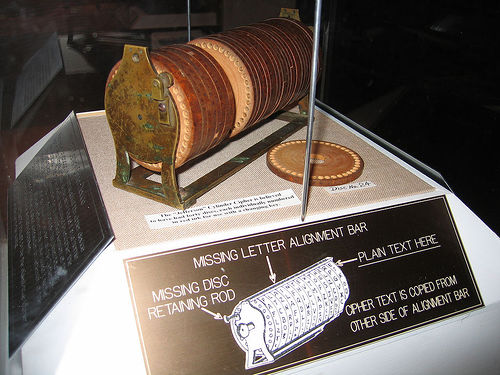
\includegraphics[width=0.4\textwidth]{images/JeffersonDisk.jpg}}
    \hspace{1.5cm}
    \subfloat[Un disque M-94, utilisé par l'armée américaine entre
1923 et 1942.]{
      \label{fig:M94}
      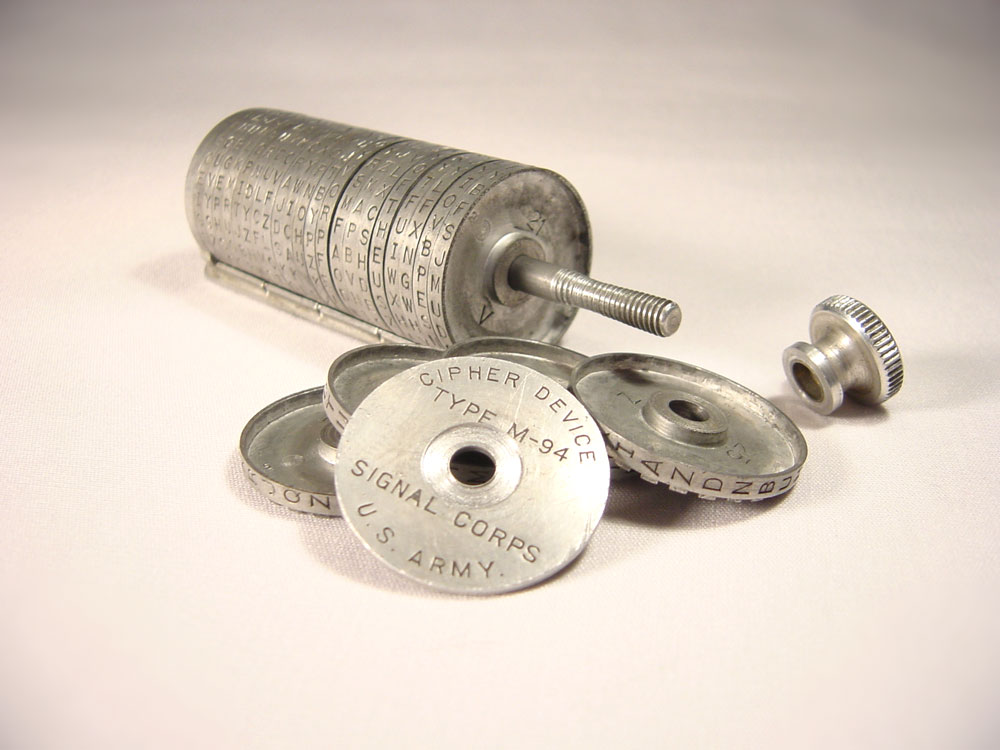
\includegraphics[width=0.4\textwidth]{images/M94.jpg}}
  \end{center}
  \vspace{-10pt}
  \caption{disques de chiffrement.}
  \vspace{-10pt}
  \label{fig:JeffersonDisks}
\end{figure}

Fin XIX\ieme, Charles Wheatstone invente un chiffre
polygrammique que nous verrons en détail plus tard~; ce chiffre
portera le nom de la personne l'ayant popularisé : le chiffre
  de Playfair. \\

Ensuite viennent plusieurs avancées cryptanalytiques avec, comme nous
l'avons vu plus haut, Charles Babbage, qui casse le chiffre de
Vigenère mais ne publie pas sa découverte. Friedrich Kasiski
le casse aussi (sans avoir connaissance des travaux de
Babbage) en 1861, et publie ses travaux. En 1891, Étienne
  Bazeries casse, quant à lui, le Grand chiffre de Louis XIV. 
\\

En 1883, Auguste Kerckhoffs publie deux articles sur la
cryptographie militaire, où il explique des règles qui peuvent être
considérées comme les règles de base d'un système cryptographique
sûr. Nous verrons ces règles en détail dans le chapitre
\ref{sec:PrincipeKerckhoffs}. \\
\clearpage
\section{La cryptographie pendant la Première Guerre mondiale}
La cryptographie était très présente pendant les guerres, d'où
l'importance des crypt\-analystes. Pour cela, chaque état avait recours
à ses cryptanalystes pour décoder les messages ennemis interceptés (ou
même alliés, c'était le cas de l'Angleterre qui écoutait les
communications entrantes et sortantes aux États-Unis).

L'organisme de déchiffrement sûrement le plus important lors de la
Première Guerre mondiale
est connu sous le nom de \emph{Room 40} (Bureau 40), le service de
déchiffrement britannique de la \emph{Royal Navy}, qui aurait déchiffré
plus ou moins 15.000 communications allemandes, la plus grosse affaire
connue étant celle du télégramme de Zimmermann.
%\begin{figure}[h]
\begin{wrapfigure}{R}{0.5\textwidth}
  \begin{center}
    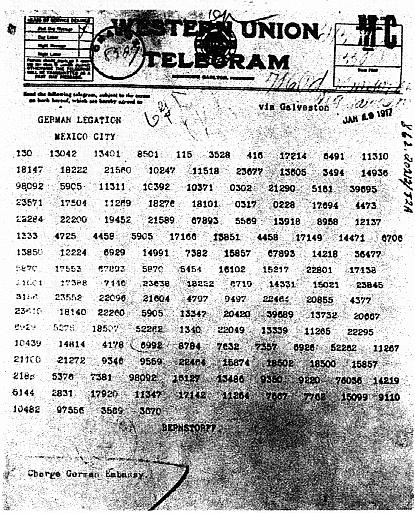
\includegraphics[width=0.48\textwidth]{images/ZimmermanTelegram.jpg}
  \end{center}
  \caption{photo du télégramme original envoyé par Zimmermann.}
  \label{fig:Zimmerman}
  \vspace{-10pt}
%\end{figure}
\end{wrapfigure}


Zimmermann était le ministre allemand des affaires étrangères durant la
guerre. En janvier 1917, alors que les États-Unis sont neutres,
Zimmermann envoya un message codé à l'ambassadeur du Mexique aux 
États-Unis. Celui-ci devait être retransmis au président mexicain après
avoir été déchiffré mais il fut intercepté par les services
secrets britanniques, qui chargèrent immédiatement le Bureau 40 du
déchiffrement du message. Un mois plus tard, c'est chose faite ; le
message indiquait que les Allemands souhaitaient déclencher une guerre
sous-marine totale et qu'il serait difficile pour les États-Unis
de rester neutres. L'Empire allemand propose alors une alliance avec le
Mexique, assorti d'une aide financière pour reconquérir le Texas, le
Nouveau-Mexique et l'Arizona. Il était aussi demandé d'essayer de
convaincre les Japonais d'entrer en guerre contre les États-Unis.
Le message fut finalement transmis au gouvernement américain après
quelques démarches évitant aux Anglais de devoir dire aux Américains
qu'ils écoutaient leurs communications diplomatiques. Le télégramme
fut publié dans la presse américaine le $1^{er}$ mars. Le 6 avril, les
États-Unis entrent en guerre contre l'Allemagne, le Congrès ayant
accepté la demande du président Wilson. Bien que la découverte du télégramme 
ne soit
pas la seule cause de l'entrée en guerre des États-Unis, il fit
fortement évoluer l'opinion publique américaine dans un sentiment
anti-allemand.

Le Bureau 40 fusionnera après la guerre avec le MI1 (département des
services secrets britanniques chargé du décryptage) pour former le
\emph{Government Code and Cypher School}, qui sera encore utile
pendant la Seconde Guerre mondiale, sous le nom de \emph{Government
  Communications Headquarters}. \\

En 1917, Gilbert Vernam invente le \emph{masque jetable}, le
seul procédé cryptographique connu comme étant à casser. Ce
procédé n'est pas directement utilisé car il pose des difficultés de
mise en place (problèmes de génération et de transmission des clés,
qui doivent être uniques) \\%TODO: voir en détail ?

%TODO: Room 40 (codebreakers, p 127 -> 150)
% Room 40 : nom du service de déchiffrement de la Royal Navy
% britannique des codes ennemis
%  déchiffré ± 15000 message
% rôle important : savoir les mouvements de la flotte allemande
% Plus grosse affaire : télégramme Zimmerman
% Fusionne avec le MI1 en 1919, sous le nom de Government Code and
% Cypher School, qui sera utile pendant la seconde WW, sous le nom de
% Government Communications Headquarters
% (MI1 : mis en place pendant la guerre, c'est le département des
% services secrets britanniques chargé du décryptage.)
% Zimmerman
% Janvier 1917, États Unis neutres
% Un message codé envoyé par Arthur Zimmerman, ministre allemand des
% affaires étrangères à destination de l'ambassade du mexique, à
% Washington
%  est intercepté par les services secrets et le room 40 est
% chargé du déchiffrement du message. Un mois après, ils y parviennent.
% Le message destiné à l'ambassadeur du mexique aux états unis
% indiquait que les allemands souhaitaient déclencher une guerre
% sous-marine totale, mais qu'il serait difficile que les états-unis
% restent neutres. L'empire allemand propose donc une alliance avec le
% mexique, qui sera aidé financièrement pour reconquérir le Texas, le
% Nouveau Mexique et l'Arizona. Le président devait aussi essayer de
% convaincre les Japonais d'entrer en guerre contre les USA.
% Le message devait être retransmit au
% président amériquain.
% Une fois ce message décodé, tout de suite envoyé aux états unis. La
% presse répand la nouvelle est les US rentrent en guerre le 6 avril
% 1917
% Ils remarquèrent que le message utilisait une technique de
% chiffrement utilisée uniquement pour les communication diplomatique
% importantes, ils se lancèrent donc d'urgence dans le déchiffrement
% du message. Le décodage fut loin d'être simple, mais le mesage
% présentait des similitudes avec d'autres messages interceptés
% auparavant. En combinant tout cela ensembles, ils réussirent petit à
% petit à décoder le message.
%TODO:image

% Chiffre de Playfair réutilisé par les Anglais
% Une version complexe du chiffre de Vigenère par les russes, cassée
% en trois jours par Hermann Pokorny
Durant la Première Guerre mondiale, de nombreux systèmes de
chiffrements utilisés étaient pour la plupart d'anciens systèmes de
chiffrements, soit réutilisés tels quels, comme le chiffre de Playfair
repris par les Anglais, soit modifiés, comme ce fut le cas
avec les russes qui utilisaient une version complexe du chiffre de
Vigenère.\\

Il en est de même pour le système de chiffrement ADFGX, inventé en
mars 1918 par le colonel allemand Fritz % TODO: lieutenant ? (kahn)
Nebel, qui combine une version modifiée
du carré de Polybe\footref{syst:CarrePolybe} (où les chiffres des
lignes et des colonnes sont remplacés par les lettres ADFGX) suivi d'une
transposition\footref{sec:Transposition} (on change la disposition
des colonnes du carré de Polybe). Les lettres ADFGX furent choisies de
façon à limiter le risque d'erreur de l'opérateur qui les
transmettrait en Morse (Nebel trouvait qu'elles étaient les lettres
les plus simples à retenir quand on apprenait le Morse).

Ce système fut déchiffré avec beaucoup de difficultés par le
lieutenant français Georges Painvin en avril de la même année, mais à
partir du mois de juin, les Allemands compliquèrent le système
cryptographique en y introduisant la lettre V (ce système se nomme
alors ADFGVX). Le tableau de $5\times 5$ cases devint alors un tableau
de $6\times 6$ cases, ce qui permit d'introduire des chiffres dans
les messages codés, et de rendre la cryptanalyse plus
compliquée.

Néanmoins, Painvin parvint à casser le code en moins de
deux jours. Cette cryptanalyse aurait permis d'arrêter l'offensive
des Allemands du printemps 1918 et aurait été une étape décisive pour
la victoire des Alliés durant cette guerre. Certains
ne sont pas d'accord et affirment que, lorsque Painvin proposa
sa solution au code, l'attaque des Allemands avait déjà échoué. 
%TODO: image explicative ?/matrice
\section{La cryptographie pendant la Seconde Guerre mondiale}
À partir des années 1920, de nombreux dispositifs mécaniques
furent mis
en place afin de faciliter le chiffrement. La plupart de ces
dispositifs se basaient sur des rotors (des disques où sont imprimées
les lettres de l'alphabet). C'est le cas de la machine \emph{Enigma},
destinée initialement aux civils (inventée en 1919 par Arthur
Scherbius et commercialisée en 1923), mais très vite utilisée par
l'armée allemande à partir des années 30. La plupart des
communications allemandes seront chiffrées via la machine Enigma, d'où
l'intérêt pour les alliés de pouvoir déchiffrer leurs messages.

La machine Enigma effectue une substitution qui change à chaque
lettre, son fonctionnement est basé sur un assemblage d'un tableau de
connection (qui ne fait que permuter quelques lettres, afin de rendre
la cryptanalyse plus difficile), de plusieurs rotors qui effectuent
les permutations des lettres, et d'un réflecteur qui renvoie le courant
sur le panneau lumineux où la lettre chiffrée s'allume. À chaque
lettre tapée, le premier rotor avance d'une position ; lorsque le
premier rotor a fait un tour complet, c'est le second qui tourne, et
ainsi de suite. Grâce à la combinaison de ces dispositifs, on peut
obtenir plus de $10^{17}$ clés possibles pour une machine à 5 rotors.

La Pologne pouvait déjà déchiffrer des messages chiffrés via Enigma en
1933 mais lorsque, 5 ans plus tard, les Allemands ajoutent deux rotors
sur les machines, les Polonais communiquent leurs travaux aux
Britanniques. Ces derniers réunissent au manoir de \emph{Bletchley
Park} des milliers de
personnes, aussi bien des mathématiciens que des linguistes, des
amateurs de mots croisés, des joueurs d'échecs professionnels ...
Cette équipe comportait notamment Alan Turing, grand mathématicien
britannique à qui on doit le concept d'ordinateur~; il s'inspire du
travail des Polonais pour créer les \emph{bombes de Turing}, qui
permettaient de retrouver le réglage de la machine à utiliser pour
déchiffrer le message, via la «~force brute~». (nous verrons ceci plus
en détail dans le chapitre \ref{chap:Cryptanalyse} sur la
cryptanalyse) \\

\begin{figure}[h]
  \begin{center}
    \subfloat[Une machine Enigma à 4 rotors.]{
      \label{fig:Enigma}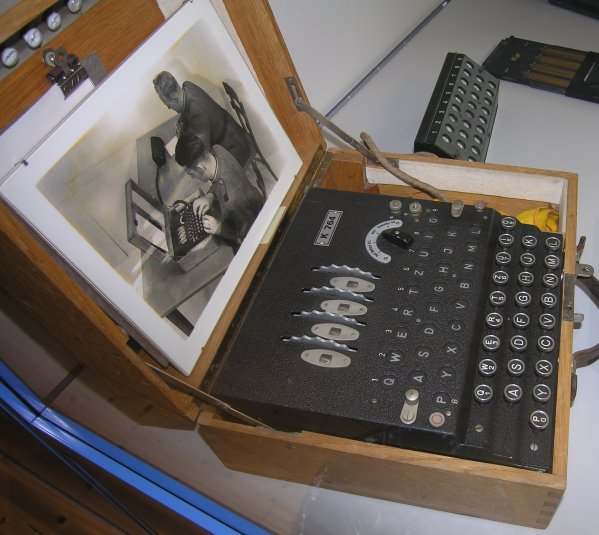
\includegraphics[width=0.4\textwidth]{images/Enigma.jpg}}
    \hspace{1.5cm}
    \subfloat[Les rotors de la Lorenz SZ42.]{
      \label{fig:Lorenz}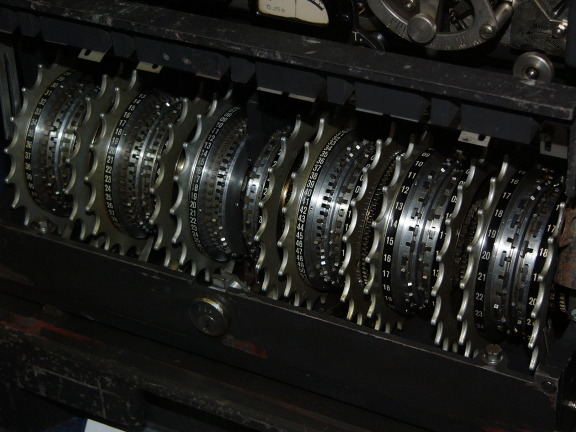
\includegraphics[width=0.4\textwidth]{images/MachineLorenz.jpg}}
  \end{center}
  \vspace{-10pt}
  \caption{machines à rotors.}
  \vspace{-10pt}
\end{figure}


Un autre code utilisé par les Allemands (pour les communications entre
les dirigeants) était le Chiffre de Lorenz, via la machine
\emph{Lorenz SZ 40} ou \emph{SZ 42}, surnommée \emph{Tunny} par les alliés. Le
Chiffre de Lorenz est en fait une application du masque jetable de
Vernam, qui nécessite une clé unique par message. Cette clé doit
être une suite de bits aléatoires (on codait les lettres en binaire
via le code Baudot, qui est une table donnant une valeur de 5 bits
pour chaque lettre de l'alphabet et certains caractères
supplémentaires). La machine de Lorenz servait donc à créer des
groupes de 5 bits aléatoires mais une machine ne peut réellement
produire un résultat aléatoire~; on parle alors de nombres
\emph{pseudo-aléatoires}.

Ce chiffre put être cassé grâce à une erreur de la part d'un opérateur
allemand, qui envoya un message de près de 4000 caractères à un autre
opérateur. Le message fut mal reçu par le second opérateur, qui
demanda de le renvoyer à nouveau. Les deux opérateurs ont alors
repositionné leur machine de Lorenz dans la même position que pour
le message d'avant, alors que le principe du masque jetable est de
n'utiliser chaque clé qu'une seule et unique fois. De plus,
l'opérateur remplaça certains mots par leur abréviation. 

Ces deux erreurs permirent à William T. Tutte, mathématicien anglais
de Bletchley Park, de trouver
facilement la clé utilisée pour ce message, de comprendre le
fonctionnement de la machine de Lorenz et de découvrir que les clés
produites n'étaient pas réellement aléatoires, ce qu'il explique dans
sa publication \emph{Fish And I}\cite{FISHAndI}.
Afin de faciliter le déchiffrement de ces messages, le
premier «~ordinateur~» électronique, le \emph{Colossus}, fut
construit. Il permettait de déchiffrer un message en quelques
heures. \\ 

Pendant que les Européens tentaient de casser Enigma et le code de
Lorenz, les Américains quant à eux travaillaient sur la machine des
Japonais, nommée \emph{97-shiki obun inji-ki} et surnommée \emph{Purple}
par les Américains. Cette machine utilisait un système proche des
rotors. William Friedman et son équipe purent reconstruire une machine
Purple à partir des messages chiffrés, en 1940, et arrivèrent à casser
les messages chiffrés des Japonais. Bien qu'ils aient décodés tous les
messages importants pendant la nuit du 6 décembre 1941, ils ne purent
éviter l'attaque de Pearl Harbor, aucun message ne disant
clairement d'attaquer à Pearl Harbor. Une alerte fut néanmoins
envoyée
à certaines bases américaines avant l'attaque, notamment à celle de
Pearl Harbor, mais ces alertes arrivèrent plusieurs heures après
l'attaque.

\section{La cryptographie moderne}
%TODO: vérifier
Après la guerre 40-45, il faudra attendre une trentaine d'années avant de
nouvelles avancées dans le domaine de la cryptologie. 

En 1971, un cryptographe d'IBM, Horst Feistel met au point un
algorithme de chiffrement par bloc, nommé \emph{Lucifer} qui
possède de nombreuses variantes. Deux ans plus tard, la NSA modifie
\emph{Lucifer} pour sortir le \emph{Data Encryption Standard},
\emph{DES}, en 1977~; il fut encore amélioré par la suite et longuement
utilisé et reste utilisé encore aujourd'hui (bien qu'il soit moins
répandu), notamment avec le \emph{Triple DES}, qui consiste
simplement à opérer trois DES consécutifs avec deux ou trois clés. %TODO: source

La même année, le chiffrement à clé publique (ou asymétrique) est
présenté pour la première fois dans une publication de W. Diffie et
M. Hellman \cite{NewDirectionsInCryptography}. Ce concept est mis en
pratique avec le chiffrement RSA, inventé par Ron Rivest, Adi Shamir
et Leonard Adleman et présenté en 1978 dans une publication 
\cite{RSAPaper}. Grâce aux algorithmes à clé publique, le problème de
distribution des clés est résolu via l'utilisation de deux clés : une
pour chiffrer, rendue publique, et une pour déchiffrer, gardée secrète
par la personne censée déchiffrer le message.

Par la suite, outre de nouveaux systèmes de chiffrements basés sur des
concepts déjà existants (comme l'\emph{International Data Encryption
  Algorithm}, un chiffrement symétrique apparu en 1990 ou le
\emph{Blowfish}, conçu par Bruce Schneier en 1993, et qui est encore
largement utilisé notemment dans
GnuPG\footnote{\url{http://www.gnupg.org}} et
OpenSSH\footnote{\url{http://www.openssh.com/}}), on peut noter
l'implémentation de la première fonction de hachage en 1989 par Ronald
Rivest, le \emph{R} du RSA, qui conçoit le \emph{Message Digest 2},
MD2 , par la suite amélioré en MD4 et MD5. L'algorithme MD5 est encore
utilisé aujourd'hui mais de moins en moins suite à des problèmes de
fiabilité. Les fonctions de hachage conseillées aujourd'hui sont les
versions récentes du \emph{Secure Hash Algorithm}, conçu par la NSA à
partir de 1993. Les fonctions de hachage sont utilisées pour vérifier
l'intégrité des données, nous verrons ceci en détail dans le chapitre
les concernant. %(chapitre \ref{sec:Hash})\\
\\

En 1990, l'idée de cryptographie quantique fait son apparition suite
aux résultats de Charles Bennet et Gilles Brassard. Elle permet, en se
basant sur les lois de la physique quantique, de distribuer des clés
en toute sécurité, afin de pouvoir utiliser un chiffre de
Vernam. Ainsi, si on met en place ce type de cryptographie, un
message pourrait devenir complètement indéchiffrable sans la clé, qui
serait impossible à trouver.

En 1991, Philip Zimmermann sort la première version de \emph{Pretty Good
  Privacy}, PGP, un logiciel de chiffrement et de signature destiné au
grand public, qui combine cryptographie symétrique et asymétrique. Il
explique très bien dans son article « Why I Wrote PGP
»\cite{WhyIWrotePGP} les raisons pour lesquelles il faut utiliser PGP,
en expliquant la volonté du gouvernement américain d'interdire toute
forme de cryptographie sauf une, afin de pouvoir surveiller les
communications du pays entier. Il en conclut qu'il faut utiliser au
maximum la cryptographie tant que c'est légal, car il est difficile de
criminaliser quelque chose de populaire, et que si la cryptographie
est mise « hors-la-loi », seuls les hors-la-loi l'utiliseront, ce qui
ne réglera pas les problèmes. Sa gratuité ayant fait son succès, ce
logiciel est encore largement
utilisé de nos jours, notamment via son implémentation libre, GnuPG. \\

Dans leur publication de 1977\cite{NewDirectionsInCryptography},
Diffie et Hellman remarquent que dans l'histoire, la plupart des
innovations cryptographiques venaient d'amateurs (les machines à
rotors, le disque de Jefferson, \dots) tandis que les professionnels
amélioraient les techniques de cryptanalyse.

Le futur de la cryptographie se tournera donc sûrement vers la
cryptographie quantique ainsi que l'allongement des clés utilisées par
les algorithmes symétriques et asymétriques.
% avec des logiciels
% combinant diverses méthodes de chiffrement (comme le fait PGP)

% La plupart des concepts et méthodes citées ou expliquées brièvement
% dans ce chapitre seront expliqués plus en détails dans les chapitres
% suivants.

% \begin{figure}[h]
%   \begin{center}
%     
\includegraphics[scale=0.2]{images/Puffy.png}
%     \hspace{1cm}
%     \includegraphics[scale=0.3]{images/BruceSchneier.jpg}
%     \hspace{1cm}
%     \includegraphics[scale=1.2]{images/PhilipZimmermann.jpg}
%   \end{center}
%   \caption{De droite à gauche : le poisson lune, emblème de
%     l'algorithme de chiffrement \emph{blowfish}, du logiciel de
%     communications sécurisées \emph{OpenSSH}, et du système
%     d'exploitation mettant l'accent sur la sécurité, \emph{OpenBSD} ;
%     Bruce Schneier, figure importante de la cryptologie actuelle,
%     inventeur de \emph{blowfish} ; Philip Zimmermann, créateur du
%     logiciel PGP}
%   \label{fig:ChiffrementSymetrique}
% \end{figure}

\section{Les chiffres de substitution}
Cette méthode consiste à simplement remplacer une lettre, un ensemble
de lettres (un \emph{polygramme}), un mot, ...  par une autre lettre,
polygramme, ou bien par un nombre ou un signe.

On peut distinguer plusieurs sortes de substitutions : 
\begin{itemize}
  \renewcommand{\makelabel}[1]{\sffamily\textbf{#1}}
  \item[Les substitutions monoalphabétiques ou simples] : 
    chaque lettre est remplacée par une autre lettre tout au long du message~; 
  \item[Les substitutions polyalphabétiques] :
    c'est en fait une combinaison de substitutions simples~;
  \item[Les substitutions polygrammiques]: 
    à la place de substituer des lettres comme le fait la substitution
    monoalphabétique, on substitue des groupes de lettres~;
  \item[Les substitutions homophoniques] : 
    chaque lettre peut être remplacée par plusieurs valeurs, choisies
    aléatoirement.
\end{itemize}

\note{Dans ce chapitre, nous ferons abstraction des caractères
  spéciaux, comme les lettres avec accents, des signes de
  ponctuations, ou autre caractères. Nous remplacerons ceux-ci par une
  espace si besoin est.}

\subsection{Les substitutions monoalphabétiques}
Ce type de substitution consiste simplement à remplacer chaque lettre
de l'alphabet par une autre lettre.

\subsubsection{Par simple décalage}
On peut par exemple, comme le fait le chiffre de
César\footref{syst:chiffrecesar}, décaler les lettres de l'alphabet d'une
clé $k$. \\

 Si nous considérons l'alphabet comme un ensemble cyclique où 
chaque lettre correspondrait à un chiffre (une fois arrivé à $Z$ ($= 25$), on 
repart de $A$ ($= 0$) $\rightarrow 25 + 1 = 0$), on peut facilement définir 
ce système de chiffrement :  \\

\definition{$e_k(c) = (c + k)~ mod~ 26$\\
  où $c$ est le caractère à chiffrer.}

Nous utilisons l'opérateur \emph{modulo}, qui nous donne le reste de
la division entière de deux entiers ($5~ mod~ 2 = 1$), ce qui nous
permet de rester dans un ensemble cyclique. \\

\paragraph{Exemple: le rot13\label{syst:rot13}}
Une application du chiffre de César est, par exemple, le \emph{ROT13},
qui est simplement un chiffre de César pour lequel la clé $k$ a une
valeur de $13$.\\

L'interêt du ROT13 réside dans le fait qu'il suffit d'appliquer deux
fois la méthode de chiffrement pour retrouver le texte en clair
($e_{13}(e_{13}(M)) = M$), ainsi, il n'y a qu'une et une seule fonction utilisée
pour le chiffrement et le déchiffrement (donc $e_{13}(x) =
d_{13}(x)$). \\

De ce fait, ROT13 n'est pas du tout pratique pour cacher des
informations, mais est parfois utilisé sur internet, dans les forums,
afin d'empêcher la lecture involontaire d'un texte (qui pourrait
dévoiler une information sur un film par exemple, et gâcherait le
plaisir au gens n'ayant pas vu le film, c'est ce qu'on appelle un 
\emph{spoiler}) 

\subsubsection{Par remplacement}
Outre le fait de décaler les lettres, on peut aussi remplacer chaque
lettre de l'alphabet par une autre lettre. Pour chiffrer, on peut alors
s'aider d'une table de substitution, comme sur la figure
\ref{fig:SubstitutionSimple}.

 \begin{figure}[h]
   \begin{center}
    \begin{tabular}{|c|c|c|c|c|c|c|c|c|c|c|c|c|c|c|c|c|c|c|c}
      \hline
      A & B & C & D & E & F & G & H & I & J & K & L & M & N & O & P &
      Q & R & S & T \\
      \hline
      A & Z & E & R & T & Y & U & I & O & P & Q & S & D & F & G & H &
      J & K & L & M \\
      \hline
    \end{tabular}
  \end{center}
  \begin{flushright}
    \begin{tabular}{c|c|c|c|c|c|}
      \hline
      U & V & W & X & Y & Z \\
      \hline
      W & X & C & V & B & N \\
      \hline
    \end{tabular}
  \end{flushright}
  \caption{Exemple simple de table de substitution}
  \label{fig:SubstitutionSimple}
\end{figure}

Dans cette table de substitution, on peut placer les lettre
aléatoirement, selon une règle, ou en utilisant une clé (qu'on notera
en début de table, et nous recopierons les caractères non utilisés par
après, voir la figure \ref{fig:SubstitutionCle}).

\begin{figure}[h]
  \begin{center}
    \begin{tabular}{|c|c|c|c|c|c|c|c|c|c|c|c|c|c|c|c|c|c|c|c}
      \hline
      A & B & C & D & E & F & G & H & I & J & K & L & M & N & O & P &
      Q & R & S & T \\
      \hline
      C & R & Y & P & T & O & A & B & D & E & F & G & H & I & J & K &
      L & M & N  & Q  \\
      \hline
    \end{tabular}
  \end{center}
  \begin{flushright}
    \begin{tabular}{c|c|c|c|c|c|}
      \hline
      U & V & W & X & Y & Z  \\
      \hline
      S & U & V & W & X & Z \\
      \hline
    \end{tabular}
  \end{flushright}
  \caption{Exemple de table de substitution avec comme clé ``crypto''}
  \label{fig:SubstitutionCle}
\end{figure}

Il existe de nombreuses méthodes dans le même genre pour remplacer
simplement une lettre par une autre, voyons en une de plus près :
\emph{le carré de Polybe.}\\

\paragraph{Exemple: le carré de Polybe\label{syst:CarrePolybe}}
Polybe est un historien grec (210 av. J.-C., 126 av. J.-C.), qui
explique vers 150 av. J.-C. une méthode de chiffrement par
substitution assez simple et intéressante.\\

Cette méthode consiste à placer les lettres de l'alphabet dans un
carré de 25 cases (il faut donc retirer une lettre, le W pour le
français, qui sera remplacé par V dans le message). La lettre chiffrée
sera remplacée par un nombre formé par le numéro de la colonne et de
la ligne de la lettre.\\

Nous pouvons représenter ce carré par une matrice de taille $5\times 5$
(voir la figure \ref{fig:Polybe}). Nous pouvons, analogiquement à la
figure \ref{fig:SubstitutionCle}, utiliser une clé pour le carré de
Polybe. \\

Le carré de Polybe est assez intéressant car il convertit les lettres
en chiffres et réduit le nombre de symbole utilisés dans le message
chiffrés (9 chiffres plutôt que 26 lettres). \\

\begin{figure}[h]
  $
  \left(
    \begin{array}{ccccc}
      A & B & C & D & E \\
      F & G & H & I & J \\
      K & L & M & N & O \\
      P & Q & R & S & T \\
      U & V & X & Y & Z
    \end{array}
  \right)
  $
  \hfill
  $
  \left(
    \begin{array}{ccccc}
      C & R & Y & P & T \\
      O & A & B & D & E \\
      F & G & H & I & J \\
      K & L & M & N & Q \\
      S & U & V & X & Z
    \end{array}
  \right)
  $
  \hfill
  $
  \left(
    \begin{array}{ccccc}
      a_{11} & a_{12} & a_{13} & a_{14} & a_{15}  \\
      a_{21} & a_{22} & a_{23} & a_{24} & a_{25}  \\
      a_{31} & a_{32} & a_{33} & a_{34} & a_{35}  \\
      a_{41} & a_{42} & a_{43} & a_{44} & a_{45}  \\
      a_{51} & a_{52} & a_{53} & a_{54} & a_{55}
    \end{array}
  \right)
  $
  \caption{Le carré de Polybe sous forme de matrice, la seconde
    matrice ayant comme clé « crypto », et la troisième représentant
    les nombres par lesquels seront remplacés les caractères dans le
    message chiffré.}
  \label{fig:Polybe}
\end{figure}

Polybe imaginait un moyen de communiquer les messages via des torches
: le nombre de torches placée à gauche correspondrait au numéro de la
ligne, et le nombre de torches à droit au numéro de la colonne. \\

Le carré de Polybe était utilisé par les nihilistes russes entre le
XIX\ieme~ et le XX\ieme~ siècle (des « terroristes » dont le but était de
% TODO: eme
tuer le tsar pour reconstruire une société sur de nouvelles
bases). Lorsqu'ils étaient attrapés et enfermés en prison, ils
communiquaient via le carré de Polybe, en donnant des coups sur les
murs. \\ %TODO: mieux expliquer

\begin{figure}[h]
  \begin{center}
    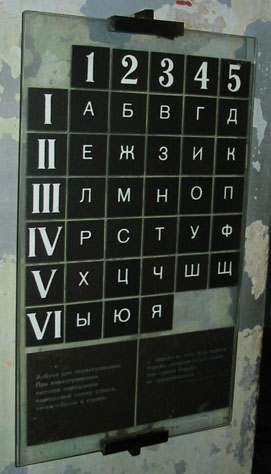
\includegraphics[scale=1.5]{eps/Nihilistes}
  \end{center}
  \caption{Version du carré de Polybe utilisée par les nihilistes
    russes}
  \label{fig:Nihilistes}
\end{figure}

\subsection{Les substitutions polyalphabétiques\label{SubstitutionPolyalphabetique}}
Les substitutions polyalphabétiques sont une combinaison de plusieurs
tables de substitutions simples, où l'on change de table à chaque
lettre, ce qui rend le message chiffré beacoup plus dur à casser sans
le code (nous verrons ceci en détail dans le chapitre
\ref{Cryptanalyse}, page \pageref{Cryptanalyse} sur la cryptanalyse)

Une des substitutions polyalphabétiques les plus connues est le
\emph{Chiffre de Vigenère}.

\paragraph{Exemple : Le chiffre de Vigenère\label{syst:ChiffreVigenere}}
Au XIX\ieme~ siècle, Vigenère « invente » une nouvelle méthode de
chiffrement en s'inspirant fortement des travaux de l'abbé allemand
Jean Trithème du XVI\ieme~ siècle. Blaise de Vigenère a néanmoins
modifié légèrement la méthode de Trithème en rendant l'utilisation de
clé de chiffrement possible.\\

La technique de Jean Trithème est d'utiliser ce qu'il décrit comme une
\emph{tabula recta}
\ref{fig:TabulaRecta}) qui est composée de 24 rangées de 24
lettres chacune. On retire donc deux lettres, le J et le V, qui seront
respectivement remplacées par le I et le W. Le W est placé après le
Z.\\
Chaque rangée correspond à un chiffre de César\footref{syst:chiffrecesar},
avec à chaque fois un décalage augmenté d'une unité. \\

Par exemple, pour chiffrer le mot « cryptographie » avec la table se
trouvant à la figure \ref{fig:TabulaRecta}~: 
\begin{itemize}
  \item la lettre C est chiffrée sur la première ligne, et reste
    donc C~;
  \item la lettre R est chiffrée sur la 2\ieme~ ligne, et devient
    S. Pour cela, trouvez la colonne de R dans la première rangée, et
    descendez d'une ligne~;
  \item La lettre Y devient W (même colonne, deux rangées plus bas)~;
  \item Et ainsi de suite ~\dots~;
  \item « cryptographie » sera donc chiffré en « csasztnwiwsur ».
\end{itemize}

\begin{figure}[h]
  \begin{center}
    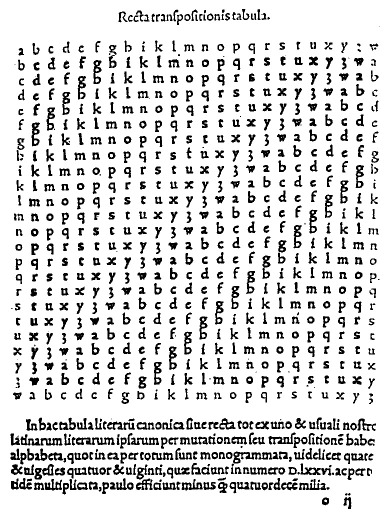
\includegraphics[scale=0.3]{eps/TabulaRecta}
  \end{center}
  \caption{La \emph{tabula recta} de Jean Trithème}
  \label{fig:TabulaRecta}
\end{figure}

Vigenère reprends donc cette méthode pour légèrement la modifier (y
ajouter l'utilisation d'une clé en fait), et la publie dans son livre
\emph{Traicté des chiffres, ou secretes
  manieres d'escrire} en 1586. \\

Comme pour la méthode de Trithème, on utilise une table, composée
cette fois ci des 26 chiffres de César possibles, comme sur la figure
\ref{fig:VigenereTableau} (Trithème en décrivait 24 dans son livre,
mais on pourrait très bien aussi en utiliser 26). \\

Expliquons cette méthode au travers d'un exemple : chiffrons « chiffre
de vigenere » avec comme mot cle « crypto ».
\begin{itemize}
  \item Tout d'abord, chaque lettre du message est associée à une
    lettre de la clé, de la façon suivante : \\
    \begin{tabular}{c@{}c@{}c@{}c@{}c@{}c@{}cc@{}cc@{}c@{}c@{}c@{}c@{}c@{}c@{}c}
      c & h & i & f & f & r & e &
      d & e &
      v & i & g & e & n & e & r & e \\

      c & r & y & p & t & o & c & 
      r & y & 
      p & t & o & c & r & y & p & t \\
    \end{tabular}\\
    La clé est donc répétée successivement~;
  \item Ensuite, chaque lettre du message clair est décalée du nombre
    de rang correspondant à la lettre de la clé qui lui est
    associée. Ainsi, pour la première lettre, C, on la décale de 2
    rangs (la lettre C lui étant associée, et la place de cette lettre
    dans l'alphabet en partant de 0 est 2). Pour s'aider, on peut
    utiliser la table du chiffre de Vigenère (voir la figure
    \ref{fig:VigenereTableau}). \\
    Ainsi, C est chiffré en E.
  \item Et on continue ainsi de suite, H est chiffré en Y, \dots
  \item « chiffre de vigenere » sera donc chiffré en « eyguyfg uc
    kbugecgx »
\end{itemize}

\begin{figure}[h]
  \begin{center}
    \begin{tabular}{c|c@{}c@{}c@{}c@{}c@{}c@{}c@{}c@{}c@{}c@{}c@{}c@{}c@{}c@{}c@{}c@{}c@{}c@{}c@{}c@{}c@{}c@{}c@{}c@{}c@{}c}
        & A & B & C & D & E & F & G & H & I & J & K & L & M & N & O & P & Q & R & S & T & U & V & W & X & Y & Z \\
      \hline
      A & A & B & C & D & E & F & G & H & I & J & K & L & M & N & O & P & Q & R & S & T & U & V & W & X & Y & Z \\
      B & B & C & D & E & F & G & H & I & J & K & L & M & N & O & P & Q & R & S & T & U & V & W & X & Y & Z & A \\
      C & C & D & E & F & G & H & I & J & K & L & M & N & O & P & Q & R & S & T & U & V & W & X & Y & Z & A & B \\
      D & D & E & F & G & H & I & J & K & L & M & N & O & P & Q & R & S & T & U & V & W & X & Y & Z & A & B & C \\
      E & E & F & G & H & I & J & K & L & M & N & O & P & Q & R & S & T & U & V & W & X & Y & Z & A & B & C & D \\
      G & G & H & I & J & K & L & M & N & O & P & Q & R & S & T & U & V & W & X & Y & Z & A & B & C & D & E & F \\
      H & H & I & J & K & L & M & N & O & P & Q & R & S & T & U & V & W & X & Y & Z & A & B & C & D & E & F & G \\
      I & I & J & K & L & M & N & O & P & Q & R & S & T & U & V & W & X & Y & Z & A & B & C & D & E & F & G & H \\
      J & J & K & L & M & N & O & P & Q & R & S & T & U & V & W & X & Y & Z & A & B & C & D & E & F & G & H & I \\
      K & K & L & M & N & O & P & Q & R & S & T & U & V & W & X & Y & Z & A & B & C & D & E & F & G & H & I & J \\
      L & L & M & N & O & P & Q & R & S & T & U & V & W & X & Y & Z & A & B & C & D & E & F & G & H & I & J & K \\
      M & M & N & O & P & Q & R & S & T & U & V & W & X & Y & Z & A & B & C & D & E & F & G & H & I & J & K & L \\
      N & N & O & P & Q & R & S & T & U & V & W & X & Y & Z & A & B & C & D & E & F & G & H & I & J & K & L & M \\
      O & O & P & Q & R & S & T & U & V & W & X & Y & Z & A & B & C & D & E & F & G & H & I & J & K & L & M & N \\
      P & P & Q & R & S & T & U & V & W & X & Y & Z & A & B & C & D & E & F & G & H & I & J & K & L & M & N & O \\
      Q & Q & R & S & T & U & V & W & X & Y & Z & A & B & C & D & E & F & G & H & I & J & K & L & M & N & O & P \\
      R & R & S & T & U & V & W & X & Y & Z & A & B & C & D & E & F & G & H & I & J & K & L & M & N & O & P & Q \\
      S & S & T & U & V & W & X & Y & Z & A & B & C & D & E & F & G & H & I & J & K & L & M & N & O & P & Q & R \\
      T & T & U & V & W & X & Y & Z & A & B & C & D & E & F & G & H & I & J & K & L & M & N & O & P & Q & R & S \\
      U & U & V & W & X & Y & Z & A & B & C & D & E & F & G & H & I & J & K & L & M & N & O & P & Q & R & S & T \\
      V & V & W & X & Y & Z & A & B & C & D & E & F & G & H & I & J & K & L & M & N & O & P & Q & R & S & T & U \\
      W & W & X & Y & Z & A & B & C & D & E & F & G & H & I & J & K & L & M & N & O & P & Q & R & S & T & U & V \\
      X & X & Y & Z & A & B & C & D & E & F & G & H & I & J & K & L & M & N & O & P & Q & R & S & T & U & V & W \\
      Y & Y & Z & A & B & C & D & E & F & G & H & I & J & K & L & M & N & O & P & Q & R & S & T & U & V & W & X \\
      Z & Z & A & B & C & D & E & F & G & H & I & J & K & L & M & N & O & P & Q & R & S & T & U & V & W & X & Y \\
    \end{tabular}
  \end{center}
  \caption{Le tableau utilisé pour le chiffre de Vigenère}
  \label{fig:VigenereTableau}
\end{figure}

Le chiffre de Vigenère consiste donc à « additionner » la lettre du
message clair à la lettre de la clé : 
\definition{$e_k(C) = C + K$}

Il existe alors de nombreuses variantes au chiffre de Vigenère qui
consistent à effectuer d'autres opérations simples avec le caractère
clair et le caractère de la clé (facilement faisable à la main) ,
comme on peut en voir quelques unes dans la table \ref{tab:VariantesVigenere}. 
\begin{table}[h]
  \caption{Quelques variantes du chiffre de Vigenère}
  \label{tab:VariantesVigenere}
  \begin{center}
    \begin{tabular}{|l|c|}
      \hline
      \textbf{Nom du chiffre} & \textbf{Opérations} \\
      \hline
      Chiffre de Vigenère & $e_k(C) = C + K$ \\ 
      \hline
      Chiffre de Beaufort & $e_k(C) = K - C$ \\
      \hline
      Chiffre de Beaufort, variante allemande & $e_k(C) = C - K$ \\
      \hline
    \end{tabular}
  \end{center}
\end{table}
%TODO: expliquer les méthodes à la main ? http://www.apprendre-en-ligne.net/crypto/menu/index.html

\subsection{Autres types de substitutions}
Il existe encore d'autres types de substitutions, comme les
substitutions homophoniques, qui, pour empêcher l'analyse des
fréquences (voir le chapitre \ref{chap:cryptanalyse} sur la
cryptanalyse), permettent de remplacer une lettre par plusieurs
symboles différents, choisis arbitrairement. On peut par exemple citer
une variante du chiffre de Vigenère, où l'on chiffre chaque lettre par
une des lettres de la même ligne suivie d'une des lettre de la même
colonne. On peut aussi utiliser des tables de substitutions, et même
varier le nombre de représentation possibles d'un symbole en fonction
de sa fréquence d'apparition (le \emph{E} pourra donc être représenté par
de nombreux symboles, ce qui ne sera pas le cas du \emph{Z}).\\

Il existe aussi des substitutions polygrammiques, où l'on ne chiffre
pas lettre par lettre, mais par polygramme, c'est à dire par ensemble
de lettre. Comme chiffre polygrammique, il existe par exemple le
chiffre de Playfair, inventé par Charles Wheatstone en 1854 et qui fut
réutilisé pendant la Première Guerre mondiale. Pour l'anecdote,
quand Wheatstone proposa au \emph{Foreign Office} --- qui trouvait son chiffre
trop compliqué pour être utiliser --- de montrer sa simplicité en
l'apprenant aux trois-quarts des enfants de l'école primaire voisine
en moins d'un quart d'heure, on lui répondit « C'est bien possible,
mais vous ne pourrez jamais l'apprendre à des spécialistes ».

Cette méthode chiffre les lettres par digrammes (par deux) en se
basant sur quatre simples règles. On utilise un tableau de $5x$ cases,
où le chiffrement se fera en fonction de la position des deux lettres
dans le tableau.  

Tout d'abord, dans le cas où les deux lettres sont
identiques, on ajoute un \emph{X} à la suite de la première
lettre. C'est aussi valable dans le cas où il ne reste qu'une lettre.
Ensuite, nous avons trois possibilités en regardant la position des
lettre dans le tableau : 
\begin{itemize}
  \item les lettres sont sur la même ligne : on les remplace par les
    lettres situées à droite (en considérant les lignes comme
    cycliques, c'est à dire que la lettre à droite de la dernière
    lettre de la ligne est la lettre située la plus à gauche) ; 
  \item les lettres sont dans la même colonne : on les remplace par la
    lettre située en dessous (en considérant aussi les colonnes comme
    cycliques)
  \item les lettre ne sont ni sur la même colonne, ni sur la même
    ligne : on remplace la lettre par celle se situant sur la même
    ligne que la lettre à chiffrer, et sur la colonne de la seconde
    lettre.
\end{itemize}

\begin{figure}[h]
  $
  \left(
    \begin{array}{ccccc}
      \textcolor{green}{\underline{C}} & \textcolor{red}{\underline{R}} & Y & \textcolor{green}{P} & \textcolor{red}{T} \\
      O & A & B & D & E \\
      F & G & H & I & J \\
      K & L & M & N & Q \\
      S & U & V & X & Z
    \end{array}
  \right)
  $
  \hfill
  $
  \left(
    \begin{array}{ccccc}
      C & \textcolor{red}{R} & Y & P & T \\
      O & A & B & D & E \\
      F & \textcolor{green}{\underline{G}} & H & I & J \\
      K & \textcolor{red}{\underline{L}} & M & N & Q \\
      S & \textcolor{green}{U} & V & X & Z
    \end{array}
  \right)
  $
  \hfill
  $
  \left(
    \begin{array}{ccccc}
      C & R & Y & P & T \\
      O & \textcolor{red}{\underline{A}} & B & \textcolor{green}{\underline{D}} & E \\
      F & G & H & I & J \\
      K & L & M & N & Q \\
      S & \textcolor{green}{U} & V & \textcolor{red}{X} & Z
    \end{array}
  \right)
  $
  \caption{Les trois règles du chiffre de Playfair, les lettre à
    chiffrer sont en vert et les lettres chiffrées en rouge. La
    première lettre du digramme est soulignée}
  \label{fig:Playfair}
\end{figure}

%\subsection{Substitution homophonique}
% Chaque lettre peut être remplacée par plusieurs lettres/chiffres
%\subsection{Substitution polygrammique}
% Subsitituions de plusieurs caractères


%\part{ Annexes}
\appendix

% Fin du travail : La bibliographie, le glossaire, à propos
\backmatter
\nocite{*}
\bibliographystyle{plain}
\bibliography{bibliographie/bibliographie}

\end{document}
